La visualisation \textit{bipartite graph} a été réalisée à partir de trois fichiers \gls{csv} provenant de la base de données du projet \gls{vhs}. 

Deux d'entre eux, les \textit{witnesses 75 et 76}, sont des témoins de l'œuvre \textit{Cyclopedia}. Il s'agit des volumes 1 et 2. Cette œuvre créée en 1728 à Londres par Ephraïm Chambers est une encyclopédie regroupant diverses savoirs en arts et science. Sa traduction en français est le point de départ de l'écriture de l'\textit{Encyclopédie} de Diderot et D'Alembert\footcite{CyclopaediaEncyclopaediaChambersa}. 

Le \textit{witness 116} est une copie du \textit{Elementa Matheseos universae} du mathématicien et philosophe Christian von Wolff. Ce dernier est considéré comme le porte-parole allemand des Lumières\footcite{ChristianBaronWolff2025}. Il est surtout connu en mathématiques pour ses manuels qui sont des références pour l'enseignement et l'apprentissage\footcite{ChristianWolffsElementaa}.

Comparer les \textit{regions} extraites de ces deux œuvres nous permet de mettre en évidence la diffusion de connaissances présentes dans des manuels de mathématiques vers des encyclopédies qui ont pour but de réunir et réorganiser tout les savoirs existants. Les images sont elles reprises telles quelles ou sont-elles simplifiées ? Y a-t-il une évolution dans les conventions de représentation ?

Pour ces trois \textit{witnesses}, les résultats de la reconnaissance automatique de similarité ont été annoté par les chercheurs. Ils offrent alors une plus grande précision, ce qui permet de mettre en évidence des similarité que l'algorithme n'aurait pas nécessairement identifiés.

La visualisation met en évidence l'existence de conventions de représentation différentes entre les images de la \textit{Cyclopedia} d'Ephraïm Chambers et celles des \textit{Elementa Matheseos universae} de Christian von Wolff. 

\begin{figure}[H]
	\centering
	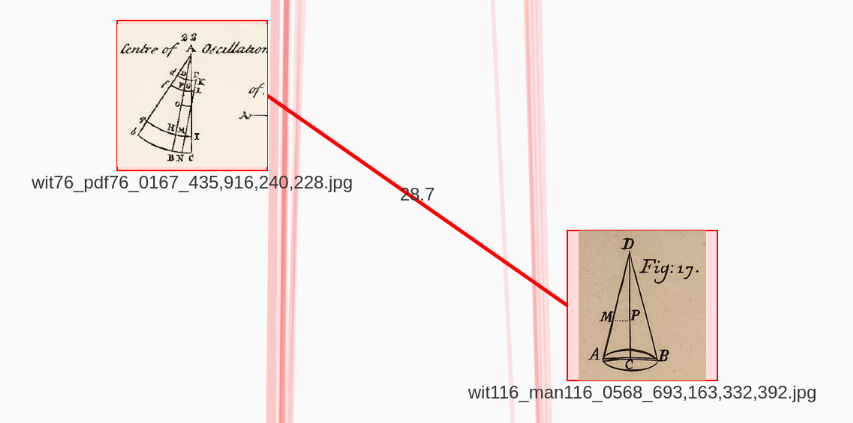
\includegraphics[width=0.8\textwidth]{images/bipartite_3.png}
	\label{fig:bipartite_3}
	\caption{Deux conventions de représentation d'un même concept}
\end{figure}

Dans cet exemple, nous pouvons observer que dans le \textit{Elementa Matheseos universae} la figure géométrique est représentée en trois dimensions alors qu'elle apparaît en deux dimensions dans la \textit{Cyclopedia}.

\begin{figure}[H]
	\centering
	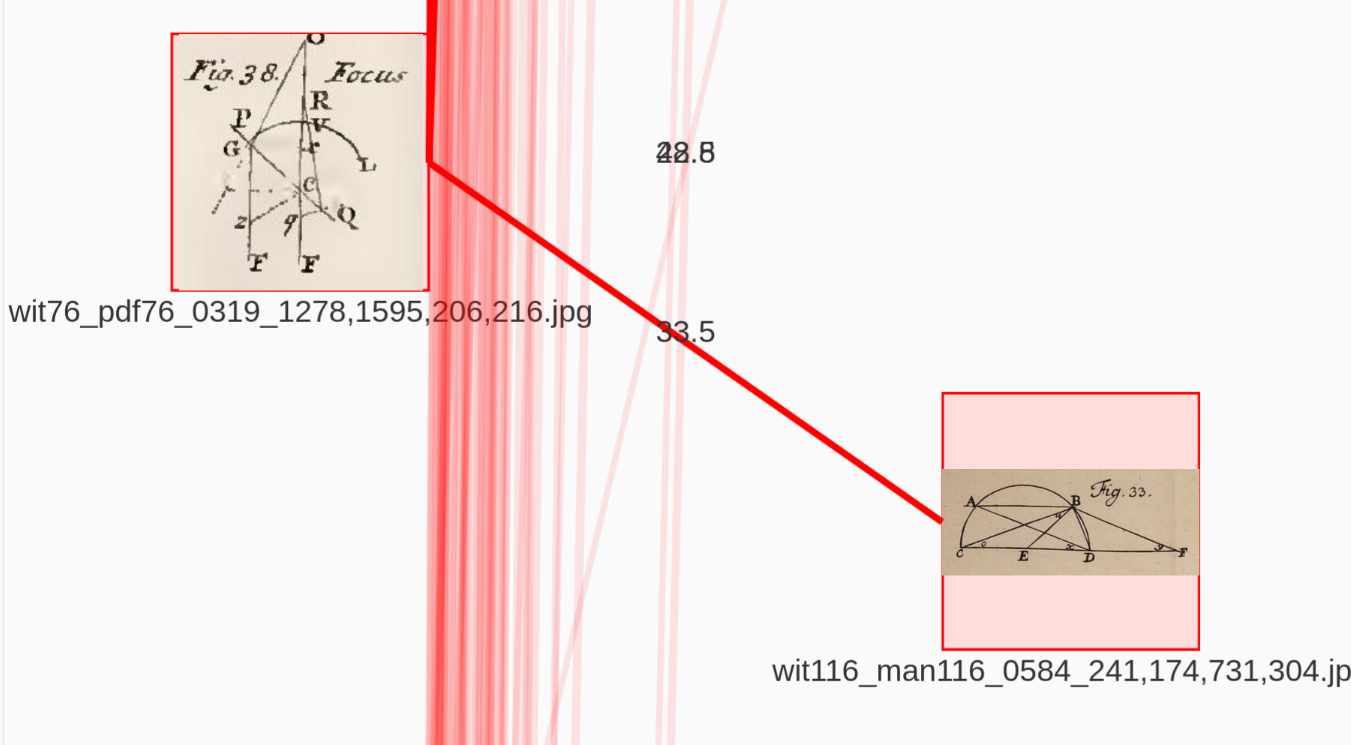
\includegraphics[width=0.8\textwidth]{images/bipartite_2.png}
	\label{fig:bipartite_2}
	\caption{Deux figures géométriques représentées légèrement différemment}
\end{figure}

Dans cet autre exemple, la figure géométrique de la \textit{Cyclopedia} est représentée dans un autre sens que celle des \textit{Elementa Matheseos universae}, ce qui a un impact direct sur le tracé des formes.